%!TEX root = doc.tex
\section{The \apiname{} API} % (fold)
\label{sec:proposal}

%% Intro to the proposal
% Framework limitations issues
The modelling of agent-based systems can be accomplished using on of the wide number of available platforms, such as those surveyed in Nikolai \emph{et al.}\cite{survey}. In order to benefit from different features, modelling the same MAS in different tools may be necessary.
% The main goal of this proposal
The API we propose is the direct result of an undergoing project to solve such necessity. More specifically, we propose a way to easily create JADE-like simulations based solely on the Repast Symphony platform.

The main feature of \apiname{} is the fact that it enables the development of FIPA-compliant MABS in Repast.
% A secondary objective
An objective that has also been taken in consideration in the framework's architecture is ultimately being able to perform a seamless conversion between the two frameworks.
% Conclusion and intro to the section objective
In this section we describe \apiname{}'s architecture thoroughly, while comparing our design decisions with those of JADE.
% [citation needed: is conversion a real need?]


%% Summarizing and comparing Repast and JADE features
%\subsection{Repast and JADE}
% What was missing in Repast?
%JADE and Repast are two popular agent-based frameworks with a very distinct set of features. Table \ref{tab:jadevsrep} summarizes the main differences between the two.

%Our goal is not to reproduce JADE's distributed architecture in Repast. One advantage of using Repast is that, since communication is local (while JADE agents are often spread in different containers), the execution of Repast-based simulations is typically much faster. This also makes it more suited to perform simulations and tests on MAS \cite{mengistu2008scalability} \cite{gormer2011jrep} \cite{garcia2011misia}.

%By incorporating FIPA specifications in Repast, we bring it closer to JADE. Also, when using \apiname{}, programmers that are already comfortable with creating MAS in JADE can feel comfortable enough to produce Repast-based simulations with the features they are used to in JADE.

\subsection{\gls{FIPA} Specifications}

% Brief intro
As previously mentioned, \apiname{} closely follows JADE's architecture and includes the four main concepts proposed by \gls{FIPA}: the \gls{DF}, the \gls{MTS}, the ACL Message and the Interaction protocols.
% The DF Agent Description
Our API implements the DF Agent Description used to filter DF searches. The focus of our tool is the development of local simulations (as opposed to distributed). As such, a single DF exists in each simulation. \apiname{}'s implementation of the MTS is simplified as well due to the absence of a distributed infrastructure; all our agents are local, therefore agent address resolution is unnecessary.

% The Repast Context
It is worth noting that Repast has its own agent manager, named ``Context''.
Repast's Context contains all objects that are to be scheduled. In \apiname{}'s this consists off all active behaviours. 

%\apiname{} offers support to this feature by integrating a reference to the Context in the DF, while preserving the API's independence from Repast. While not present in JADE, this feature was included in \apiname{} out of convenience and is used internally. 

Our implementation uses a version of the ACL Message that is slightly simpler than in the one found in JADE, focusing on the most common elements (the ones highlighted in Table \ref{tab:fipaACLMessage}).

Finally, the main focus of the API we're proposing is the incorporation of \gls{FIPA} Interaction Protocols in Repast. At the present time, we chose to include a few of the most common protocols in \apiname{}, following JADE's implementation.

The \gls{FIPA} protocols from JADE we chose to include in \apiname{} at this point were the ``request-like'' Achieve Rational Effect (AchieveRE) protocol, the Propose protocol and the Contract Net protocol. The AchieveRE is a single protocol that encompasses multiple \gls{FIPA} protocols, namely FIPA-Request, FIPA-query, FIPA-Request-When, FIPA-recruiting and FIPA-brokering protocols, as defined in JADE's documentation \footnote{http://jade.tilab.com/doc/api/jade/proto/AchieveREInitiator.html}.


\subsection{Agent Execution}

In the process of integrating JADE's protocols in \apiname{}, it was necessary to make adaptations to its behaviours' implementation in order to take Repast's concept of time into account. Even though a local application can take advantage of direct method invocation, for the sake of compatibility with JADE communication in \apiname{} is made asynchronously.

JADE agent execution is concurrent and possibly parallel, since JADE supports distributed and multi-threaded agent systems. Agent execution in Repast, on the other hand, in not concurrent. Repast uses a time-share type of execution, granting each agent the right to perform its tasks until they finish them, in sequence, but in no particular order.

Figures \ref{fig:com-example-jade} and \ref{fig:com-example-repast} represent a scenario where two agents send a message to a third one, who then replies to the first two. In Repast, messages are delivered to the agent's mailbox, and processed later on while in JADE, messages can arrive concurrently and be processed right away, because the arrival of a message triggers a correspondent event.

\begin{figure}
	\centering
	\includegraphics[width=3.0in]{figures/tickExample2.pdf}
	\caption{
		Communication example in JADE. Agents are executed concurrently or in parallel. Agent C tries to handle messages as they arrive and issues the respective reply.
	}
	\label{fig:com-example-jade}
\end{figure}

\begin{figure}
	\centering
	\includegraphics[width=3.5in]{figures/tickExample.pdf}
	\caption{
		Communication example in Repast using \apiname{} in a single tick. In their respective turns, A and B send a message to C, which stays in standby in C's Mailbox. Only in C's turn do these messages get handled.
	}
	\label{fig:com-example-repast}
\end{figure}

It is worth noting that the order by which Repast executes each scheduled behaviour is never guaranteed. In fact, it is not guaranteed that all the behaviours of a single agent are executed together. This is the expected execution when working with Repast as well as with JADE and it is up to the programmer to ensure that the application does not depend on the order or execution.

\subsection{Architecture}

Figure \ref{fig:arch} illustrates the details of \apiname{}'s architecture. Most concepts represented in this diagram are present in JADE, namely the Agent, ACL Message, Behaviour, MTS and DF service.

An agent in \apiname{} contains a set of Behaviours and a Mail Box. The Behaviours have access to the agent who owns them and to its Mail Box. A behaviour tha implements an interaction protocol contains a Message Template which is used in the Mail Box to retrieve relevant messages.

The DF Service, as described before, provides the yellow page service. Agents can register or unregister themselves in the DF as well as perform searches. While tasks can be performed during agent setup, in runtime they are typically executed inside Behaviours.

To follow JADE-like communication, ACL Messages carry agent identifiers (AID) for senders and receivers. These AIDs are returned by the DF as search results and are resolved to an agent by the MTS when sending a message.

The ``plug-in points'' to the API are the Agent and the Behaviour and its derived classes. In Figure \ref{fig:arch}, all protocol definitions are implied by the generic sub-classes ``ProtocolInitiator'' and ``ProtocolResponder''.

\begin{figure}
	\centering
	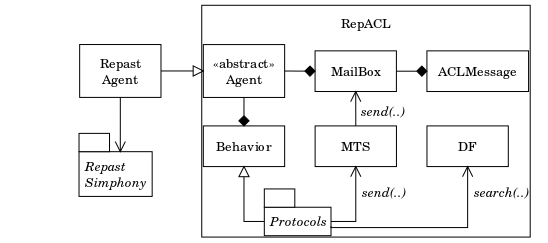
\includegraphics[width=\linewidth]{figures/repacl_arch.pdf}
	\caption{Detailed architecture or \apiname{}}
	\label{fig:arch}
\end{figure}

\subsection{Using Repast}

The Context is an utility created to provide support for Repast. In order for the simulation to run, scheduled behaviours must be added to it. In Repast simulations, the context must be set in the API by the Context Builder, which functions as the main class of a Repast simulation. We decided to integrate this feature in \apiname{} despite not being present in JADE to preserve the API's independence from Repast. This way, \apiname{} has it's own internal representation of the context.

Repast uses Java annotations to indicate which methods are to be scheduled. \apiname{}'s Behaviours contain an \texttt{action} method that should be scheduled and called when programmers implement their own instances of the Behaviours in the API. The following Java snippet represents the basic recommended usages of the Repast scheduler when extending \apiname{}'s Behaviours. Being a Repast construct, the action method is not used for actual behaviour tasks.

\begin{lstlisting}[language=Java]
	public class MyBehaviour extends Behaviour {
		...
		@Override
		@ScheduledMethod(start=1, interval=0.1)
		public void action() {
			super.action();
		}
		...
	}
\end{lstlisting}


% section proposal (end)